\documentclass{article} % For LaTeX2e
\usepackage{nips14submit_e,times}
\usepackage{amsmath}
\usepackage{amsthm}
\usepackage{amssymb}
\usepackage{mathtools}
\usepackage{hyperref}
\usepackage{url}
\usepackage{algorithm}
\usepackage[noend]{algpseudocode}
%\documentstyle[nips14submit_09,times,art10]{article} % For LaTeX 2.09

\usepackage{graphicx}
\usepackage{caption}
\usepackage{subcaption}
\usepackage{tikz-cd}

\def\eQb#1\eQe{\begin{eqnarray*}#1\end{eqnarray*}}
\def\eQnb#1\eQne{\begin{eqnarray}#1\end{eqnarray}}
\providecommand{\e}[1]{\ensuremath{\times 10^{#1}}}
\providecommand{\pb}[0]{\pagebreak}
\DeclarePairedDelimiter\ceil{\lceil}{\rceil}
\DeclarePairedDelimiter\floor{\lfloor}{\rfloor}

\newcommand{\E}{\mathrm{E}}
\newcommand{\Var}{\mathrm{Var}}
\newcommand{\Cov}{\mathrm{Cov}}

\def\Qb#1\Qe{\begin{question}#1\end{question}}
\def\Sb#1\Se{\begin{solution}#1\end{solution}}

\newenvironment{claim}[1]{\par\noindent\underline{Claim:}\space#1}{}
\newtheoremstyle{quest}{\topsep}{\topsep}{}{}{\bfseries}{}{ }{\thmname{#1}\thmnote{ #3}.}
\theoremstyle{quest}
\newtheorem*{definition}{Definition}
\newtheorem*{theorem}{Theorem}
\newtheorem*{lemma}{Lemma}
\newtheorem*{question}{Question}
\newtheorem*{preposition}{Preposition}
\newtheorem*{exercise}{Exercise}
\newtheorem*{challengeproblem}{Challenge Problem}
\newtheorem*{solution}{Solution}
\newtheorem*{remark}{Remark}
\usepackage{verbatimbox}
\usepackage{listings}
\usepackage{mathrsfs}
\title{DiffGeoI: \\
Problem Set I}


\author{
Youngduck Choi \\
CIMS \\
New York University\\
\texttt{yc1104@nyu.edu} \\
}


% The \author macro works with any number of authors. There are two commands
% used to separate the names and addresses of multiple authors: \And and \AND.
%
% Using \And between authors leaves it to \LaTeX{} to determine where to break
% the lines. Using \AND forces a linebreak at that point. So, if \LaTeX{}
% puts 3 of 4 authors names on the first line, and the last on the second
% line, try using \AND instead of \And before the third author name.

\newcommand{\fix}{\marginpar{FIX}}
\newcommand{\new}{\marginpar{NEW}}

\nipsfinalcopy % Uncomment for camera-ready version

\begin{document}


\maketitle

\begin{abstract}
This work contains solutions to the exercises of the problem set I.
\end{abstract}

\bigskip

\begin{question}[1]
\hfill
\begin{figure}[h!]
  \centering
    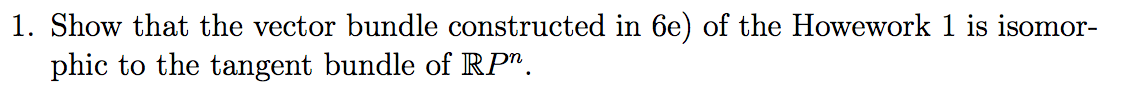
\includegraphics[width=0.7\textwidth]{DG-e3-p1.png}
\end{figure}
\end{question}
\begin{solution} \hfill \\
Consider $\mathbb{RP}^n$ as a quotient space of $S^n$, where you identify
the antipodal points. Let $p$ be the natural projection from $S^n$ to $\mathbb{RP}^n$.
For any $x \in S^n$, we have
\eQb
T_x(S^n) &=& \{ (x,v) \in S^n \times \mathbb{R}^{n+1} : x \cdot v = 0\}.
\eQe
Further observe that $(x,v)$ and $(-x,-v)$ both maps to $T_{[x]}\mathbb{RP}^n$
via the tangent map. Also, $p$ is a local diffeomorphism, so $T_p(x)$ is an isomorphism
for each $x \in S^n$. Hence, we can identify $E'$ with $T\mathbb{RP}^{n}$ via 
$f$ which sends $T_{[x]}\mathbb{RP}^{n}$ to  $([x],y)$, so we are done. \hfill
\qed 

\end{solution}

\bigskip

\begin{question}[2]
\hfill
\begin{figure}[h!]
  \centering
    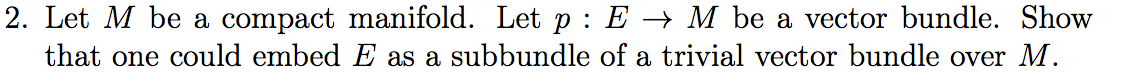
\includegraphics[width=0.7\textwidth]{DG-e3-p2.png}
\end{figure}
\end{question}
\begin{solution} \hfill \\
Let $\{U_x\}_{x \in B}$ be a collection of trivializing open sets in $B$. By 
Urysohn's lemma, there exists $\psi_x:B \to [0,1]$ such that $\psi_x$ vanishes
outside of $U_x$ and is nonzero at $x$. Consider $\{\psi_x^{-1}((0,1])\}$ 
as an open cover of $B$ and via compactness choose the finite subcover. We index
the corresponding trivializing open sets and the Urysohn functions as $\{ 
U_i, \psi_i\}$. We now define $f_i:E \to \mathbb{R}^n$ by 
\eQb
v &\mapsto& \psi_i(p(v))(\pi_i \phi_i(v))
\eQe 
where $\phi_i$ is the local trivialization of $U_i$ and $\pi_i$ is the 
projection from $M \times \mathbb{R}^n$ to $\mathbb{R}^n$. It follows that
$f_i$ is a linear inection on each fiber over $\psi_i^{-1}((0,1])$, so 
$f = (f_1,...,f_n)$ is a linear injection on each fiber which maps $E$ to 
some $\mathbb{R}^{k}$. Finally, take $h:E \to B \mathbb{R}^k$ by
first coordinate being $p$ and the second coordiate $g$. Then, the image of 
$h$ is a subbundle of $B \times \mathbb{R}^k$, since each $\mathbb{R}^n$ factor 
corresponds to the second coordinate of 
local trivialization over $\psi_i^{-1}((0,1])$.
This is the type-1 vector bundle isomorphism from $E$ to a subbundle of $B 
\times \mathbb{R}^k$, and since local trivializations are all diffeomorphism
this does give a smooth embedding in a precise sense,  so we are done. \hfill $\qed$


\end{solution}

\newpage

\begin{question}[3]
\hfill
\begin{figure}[h!]
  \centering
    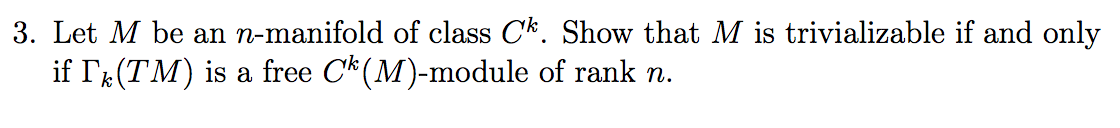
\includegraphics[width=0.7\textwidth]{DG-e3-p3.png}
\end{figure}
\end{question}
\begin{solution} \hfill \\
This statement essentially boils down to the equivalaence between a local
trivalization and local frame of a vector bundle. Obviously, we view the
tangent bundle $TM$ as a vector bundle, and the $C_k$ vector fields as
$C_k$ sections. 

\bigskip

We elaborate on the equivalence more precisely. Let $\{e_i\}$ be a fixed basis
for a typical fiber $V$. 
If $\phi$
is a local trivialization over $U$ open, then by defining 
$\sigma_i(p) = \phi^{-1}(p,e_i)$, gives $\sigma_{\phi} = (\sigma_1,...,\sigma_k)$
as a local frame over $U$. Conversely, if $\sigma_{\phi} = (\sigma_1,...,\sigma_k)$
is a local frame over $U$, then for any $v \in \pi^{-1}(U)$ has the form $v
= \sum v^{i} \sigma_{i}(p)$ for unique elements. Then, $f:U \times V \to \pi^{-1}
(U)$ defined by $(p,v) \mapsto \sum v^{i} \sigma_i(p)$ is a diffeomorphism, so 
$\sigma = f^{-1}$ is the desired trivialization. Therefore, if we have a global 
frame field, then we obtain a gloal trivalization, so the vector bundle is 
trivial.  

\bigskip 

Suppose $\Gamma_{k}(TM)$ is a free $C^k(M)-$module of rank $n$. Then,
there exists $\{e_1, ..., e_n\}$ such that, for any $ X \in \Gamma_k(TM)$,
there exists unique $f_1,...,f_n \in C^k(M)$ such that  
\eQb
X_p = f_1(p) e_1(p) + ... + f_n(p) e_n(p) \in T_{p}(M) \>\>\> (*)
\eQe 
for any $p \in M$. We claim that $\{e_1,...,e_n\}$ are global frame field. Let 
$p \in M$, and $\pi^{-1}(p) = \{p\} \times T_{p}(M)$. Fix $(p,v) \in \{p\} 
\times T_{p}(M)$. By lemma $2.65$ in Jeff M. Lee's book, there exists $X \in 
\gamma^{k}(TM)$ such that $X_p = v$. By (*), we see that $v$ can be
expressed as a linear combination of $\{e_1(p), ..., e_n(p)\}$. Since $(p,v)$
were arbitrary, we see that $\{e_1, ..., e_n\}$ is a global frame field, and
by the above discussion this implies that $TM$ is trivializable. 

\bigskip



Suppose $M$ is trivializable, thus the tangent bundle $TM$ is trivializable.
This means that $TM$ is vector bundle isomorphic to the product vector bundle 
$pr_1: M \times V \to M$. Since this is equvialent to an existence of vector bundle 
trivialization over the entire manifold $M$ (pg. 271; Jeff Lee), 
we can choose a global vector bundle trivizialization of $TM$, which we denote as $\phi$
Then, as motivated from above, set $\sigma_i(p) = \phi^{-1}(p,e_i)$, where $e_i$s
are the basis of the typical fiber. Vary $p$, to obtain $\{\sigma_i\}$ 
that are $C^k$ sections on $TM$. Now, let $X \in \Gamma_k(TM)$. Then, 
from $\sigma_i(p) = \phi^{-1}(p,e_i)$, we see that $X$ can be uniquely expressed
as a linear combination of $\{\sigma_i\}$, so $\Gamma_k(TM)$ is free. \hfill
$\qed$    
 

\end{solution}

\end{document}
